\documentclass[tikz,border=4pt]{standalone}
\usepackage[T1]{fontenc}
\usepackage{lmodern}
\usepackage{amsmath,amssymb}
\usetikzlibrary{arrows.meta,calc,positioning}

\definecolor{bgpaper}{RGB}{245,246,248}
\definecolor{ink}{RGB}{52,66,86}
\definecolor{frame}{RGB}{156,163,173}
\definecolor{headfill}{RGB}{230,233,238}
\definecolor{panelfill}{RGB}{236,238,241}
\definecolor{keptA}{RGB}{80,132,195}
\definecolor{resA}{RGB}{236,149,63}
\definecolor{ok}{RGB}{48,145,101}

\tikzset{
  panel/.style={draw=frame,fill=panelfill,line width=0.85pt,rounded corners=0.03cm},
  subpanel/.style={draw=frame!95,fill=white,line width=0.75pt},
  headline/.style={font=\bfseries\fontsize{7.0}{7.3}\selectfont},
  sechead/.style={font=\bfseries\fontsize{6.8}{7.1}\selectfont},
  cardhead/.style={font=\bfseries\fontsize{6.0}{6.3}\selectfont},
  cardsub/.style={font=\bfseries\itshape\fontsize{5.4}{5.7}\selectfont},
  celltxt/.style={font=\fontsize{5.7}{6.0}\selectfont},
  tinytxt/.style={font=\fontsize{4.7}{5.0}\selectfont},
  arrow/.style={-{Stealth[length=3.2mm,width=2.5mm]},line width=1.0pt,draw=ink}
}

\begin{document}
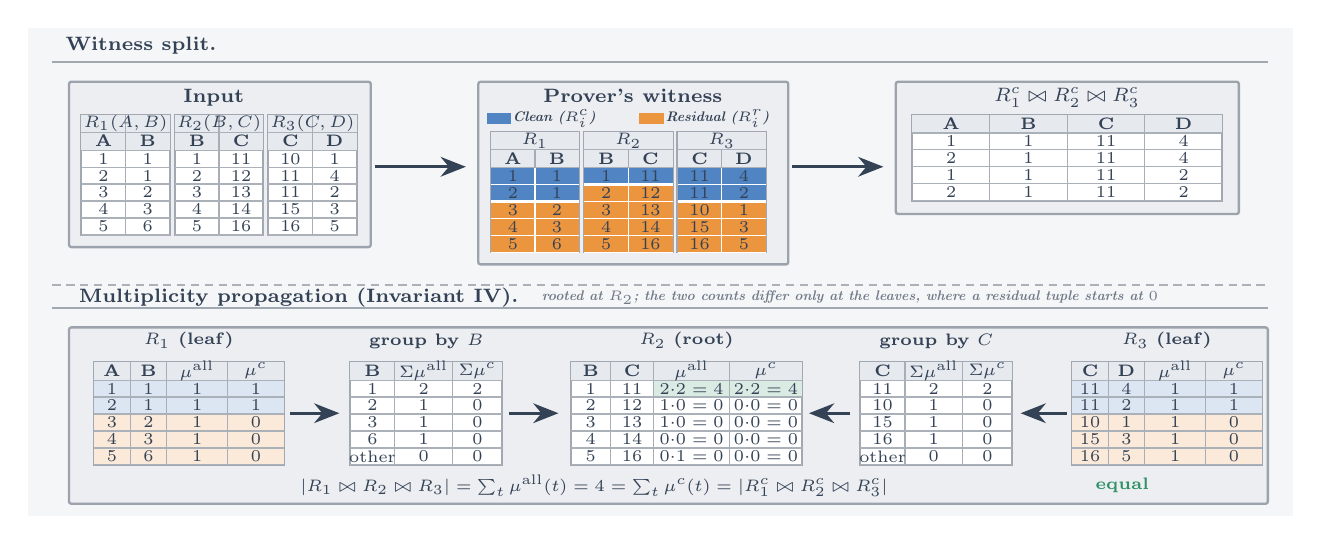
\begin{tikzpicture}[x=1.05cm,y=1cm,font=\sffamily,text=ink]

\fill[bgpaper] (0.15,-0.50) rectangle (15.45,-6.69);
\node[headline] at (1.52,-0.72) {Witness split.};
\draw[frame!95,line width=0.8pt] (0.45,-0.93) -- (15.15,-0.93);

% --- (a) Input
\draw[panel] (0.65,-1.18) rectangle (4.30,-3.28);
\node[sechead] at (2.40,-1.38) {Input};
\draw[subpanel] (0.800,-1.600) rectangle (1.870,-3.125);
\fill[headfill] (0.800,-1.600) rectangle (1.870,-2.050);
\draw[frame!88,line width=0.45pt] (1.335,-1.600) -- (1.335,-3.125);
\draw[frame!85,line width=0.45pt] (0.800,-1.820) -- (1.870,-1.820);
\draw[frame!85,line width=0.45pt] (0.800,-2.050) -- (1.870,-2.050);
\draw[frame!85,line width=0.45pt] (0.800,-2.265) -- (1.870,-2.265);
\draw[frame!85,line width=0.45pt] (0.800,-2.480) -- (1.870,-2.480);
\draw[frame!85,line width=0.45pt] (0.800,-2.695) -- (1.870,-2.695);
\draw[frame!85,line width=0.45pt] (0.800,-2.910) -- (1.870,-2.910);
\draw[frame!85,line width=0.45pt] (0.800,-3.125) -- (1.870,-3.125);
\node[cardhead] at (1.335,-1.710) {$R_1(A,B)$};
\node[cardhead] at (1.068,-1.935) {A};
\node[cardhead] at (1.603,-1.935) {B};
\node[celltxt] at (1.068,-2.158) {1};
\node[celltxt] at (1.603,-2.158) {1};
\node[celltxt] at (1.068,-2.373) {2};
\node[celltxt] at (1.603,-2.373) {1};
\node[celltxt] at (1.068,-2.588) {3};
\node[celltxt] at (1.603,-2.588) {2};
\node[celltxt] at (1.068,-2.803) {4};
\node[celltxt] at (1.603,-2.803) {3};
\node[celltxt] at (1.068,-3.018) {5};
\node[celltxt] at (1.603,-3.018) {6};
\draw[subpanel] (1.930,-1.600) rectangle (3.000,-3.125);
\fill[headfill] (1.930,-1.600) rectangle (3.000,-2.050);
\draw[frame!88,line width=0.45pt] (2.465,-1.600) -- (2.465,-3.125);
\draw[frame!85,line width=0.45pt] (1.930,-1.820) -- (3.000,-1.820);
\draw[frame!85,line width=0.45pt] (1.930,-2.050) -- (3.000,-2.050);
\draw[frame!85,line width=0.45pt] (1.930,-2.265) -- (3.000,-2.265);
\draw[frame!85,line width=0.45pt] (1.930,-2.480) -- (3.000,-2.480);
\draw[frame!85,line width=0.45pt] (1.930,-2.695) -- (3.000,-2.695);
\draw[frame!85,line width=0.45pt] (1.930,-2.910) -- (3.000,-2.910);
\draw[frame!85,line width=0.45pt] (1.930,-3.125) -- (3.000,-3.125);
\node[cardhead] at (2.465,-1.710) {$R_2(B,C)$};
\node[cardhead] at (2.197,-1.935) {B};
\node[cardhead] at (2.732,-1.935) {C};
\node[celltxt] at (2.197,-2.158) {1};
\node[celltxt] at (2.732,-2.158) {11};
\node[celltxt] at (2.197,-2.373) {2};
\node[celltxt] at (2.732,-2.373) {12};
\node[celltxt] at (2.197,-2.588) {3};
\node[celltxt] at (2.732,-2.588) {13};
\node[celltxt] at (2.197,-2.803) {4};
\node[celltxt] at (2.732,-2.803) {14};
\node[celltxt] at (2.197,-3.018) {5};
\node[celltxt] at (2.732,-3.018) {16};
\draw[subpanel] (3.060,-1.600) rectangle (4.130,-3.125);
\fill[headfill] (3.060,-1.600) rectangle (4.130,-2.050);
\draw[frame!88,line width=0.45pt] (3.595,-1.600) -- (3.595,-3.125);
\draw[frame!85,line width=0.45pt] (3.060,-1.820) -- (4.130,-1.820);
\draw[frame!85,line width=0.45pt] (3.060,-2.050) -- (4.130,-2.050);
\draw[frame!85,line width=0.45pt] (3.060,-2.265) -- (4.130,-2.265);
\draw[frame!85,line width=0.45pt] (3.060,-2.480) -- (4.130,-2.480);
\draw[frame!85,line width=0.45pt] (3.060,-2.695) -- (4.130,-2.695);
\draw[frame!85,line width=0.45pt] (3.060,-2.910) -- (4.130,-2.910);
\draw[frame!85,line width=0.45pt] (3.060,-3.125) -- (4.130,-3.125);
\node[cardhead] at (3.595,-1.710) {$R_3(C,D)$};
\node[cardhead] at (3.328,-1.935) {C};
\node[cardhead] at (3.863,-1.935) {D};
\node[celltxt] at (3.328,-2.158) {10};
\node[celltxt] at (3.863,-2.158) {1};
\node[celltxt] at (3.328,-2.373) {11};
\node[celltxt] at (3.863,-2.373) {4};
\node[celltxt] at (3.328,-2.588) {11};
\node[celltxt] at (3.863,-2.588) {2};
\node[celltxt] at (3.328,-2.803) {15};
\node[celltxt] at (3.863,-2.803) {3};
\node[celltxt] at (3.328,-3.018) {16};
\node[celltxt] at (3.863,-3.018) {5};
\draw[arrow] (4.35,-2.26) -- (5.45,-2.26);

% --- (b) Prover witness
\draw[panel] (5.60,-1.18) rectangle (9.35,-3.50);
\node[sechead] at (7.47,-1.36) {Prover's witness};
\fill[keptA] (5.70,-1.58) rectangle (6.00,-1.72);
\node[cardsub,anchor=west] at (5.90,-1.65) {Clean ($R_i^c$)};
\fill[resA] (7.55,-1.58) rectangle (7.85,-1.72);
\node[cardsub,anchor=west] at (7.75,-1.65) {Residual ($R_i^r$)};
\draw[subpanel] (5.750,-1.820) rectangle (6.820,-3.345);
\fill[headfill] (5.750,-1.820) rectangle (6.820,-2.270);
\fill[keptA] (5.750,-2.270) rectangle (6.820,-2.485);
\fill[keptA] (5.750,-2.485) rectangle (6.820,-2.700);
\fill[resA] (5.750,-2.700) rectangle (6.820,-2.915);
\fill[resA] (5.750,-2.915) rectangle (6.820,-3.130);
\fill[resA] (5.750,-3.130) rectangle (6.820,-3.345);
\draw[frame!90,line width=0.45pt] (6.285,-2.040) -- (6.285,-2.270);
\draw[white,line width=0.45pt] (6.285,-2.270) -- (6.285,-3.345);
\draw[frame!85,line width=0.45pt] (5.750,-2.040) -- (6.820,-2.040);
\draw[frame!85,line width=0.45pt] (5.750,-2.270) -- (6.820,-2.270);
\draw[white,line width=0.45pt] (5.750,-2.485) -- (6.820,-2.485);
\draw[white,line width=0.45pt] (5.750,-2.700) -- (6.820,-2.700);
\draw[white,line width=0.45pt] (5.750,-2.915) -- (6.820,-2.915);
\draw[white,line width=0.45pt] (5.750,-3.130) -- (6.820,-3.130);
\draw[white,line width=0.45pt] (5.750,-3.345) -- (6.820,-3.345);
\draw[white,line width=0.8pt] (5.750,-2.700) -- (6.820,-2.700);
\node[cardhead] at (6.285,-1.930) {$R_1$};
\node[cardhead] at (6.018,-2.155) {A};
\node[cardhead] at (6.553,-2.155) {B};
\node[celltxt] at (6.018,-2.377) {1};
\node[celltxt] at (6.553,-2.377) {1};
\node[celltxt] at (6.018,-2.592) {2};
\node[celltxt] at (6.553,-2.592) {1};
\node[celltxt] at (6.018,-2.808) {3};
\node[celltxt] at (6.553,-2.808) {2};
\node[celltxt] at (6.018,-3.022) {4};
\node[celltxt] at (6.553,-3.022) {3};
\node[celltxt] at (6.018,-3.237) {5};
\node[celltxt] at (6.553,-3.237) {6};
\draw[subpanel] (6.880,-1.820) rectangle (7.950,-3.345);
\fill[headfill] (6.880,-1.820) rectangle (7.950,-2.270);
\fill[keptA] (6.880,-2.270) rectangle (7.950,-2.485);
\fill[resA] (6.880,-2.485) rectangle (7.950,-2.700);
\fill[resA] (6.880,-2.700) rectangle (7.950,-2.915);
\fill[resA] (6.880,-2.915) rectangle (7.950,-3.130);
\fill[resA] (6.880,-3.130) rectangle (7.950,-3.345);
\draw[frame!90,line width=0.45pt] (7.415,-2.040) -- (7.415,-2.270);
\draw[white,line width=0.45pt] (7.415,-2.270) -- (7.415,-3.345);
\draw[frame!85,line width=0.45pt] (6.880,-2.040) -- (7.950,-2.040);
\draw[frame!85,line width=0.45pt] (6.880,-2.270) -- (7.950,-2.270);
\draw[white,line width=0.45pt] (6.880,-2.485) -- (7.950,-2.485);
\draw[white,line width=0.45pt] (6.880,-2.700) -- (7.950,-2.700);
\draw[white,line width=0.45pt] (6.880,-2.915) -- (7.950,-2.915);
\draw[white,line width=0.45pt] (6.880,-3.130) -- (7.950,-3.130);
\draw[white,line width=0.45pt] (6.880,-3.345) -- (7.950,-3.345);
\draw[white,line width=0.8pt] (6.880,-2.485) -- (7.950,-2.485);
\node[cardhead] at (7.415,-1.930) {$R_2$};
\node[cardhead] at (7.147,-2.155) {B};
\node[cardhead] at (7.683,-2.155) {C};
\node[celltxt] at (7.147,-2.377) {1};
\node[celltxt] at (7.683,-2.377) {11};
\node[celltxt] at (7.147,-2.592) {2};
\node[celltxt] at (7.683,-2.592) {12};
\node[celltxt] at (7.147,-2.808) {3};
\node[celltxt] at (7.683,-2.808) {13};
\node[celltxt] at (7.147,-3.022) {4};
\node[celltxt] at (7.683,-3.022) {14};
\node[celltxt] at (7.147,-3.237) {5};
\node[celltxt] at (7.683,-3.237) {16};
\draw[subpanel] (8.010,-1.820) rectangle (9.080,-3.345);
\fill[headfill] (8.010,-1.820) rectangle (9.080,-2.270);
\fill[keptA] (8.010,-2.270) rectangle (9.080,-2.485);
\fill[keptA] (8.010,-2.485) rectangle (9.080,-2.700);
\fill[resA] (8.010,-2.700) rectangle (9.080,-2.915);
\fill[resA] (8.010,-2.915) rectangle (9.080,-3.130);
\fill[resA] (8.010,-3.130) rectangle (9.080,-3.345);
\draw[frame!90,line width=0.45pt] (8.545,-2.040) -- (8.545,-2.270);
\draw[white,line width=0.45pt] (8.545,-2.270) -- (8.545,-3.345);
\draw[frame!85,line width=0.45pt] (8.010,-2.040) -- (9.080,-2.040);
\draw[frame!85,line width=0.45pt] (8.010,-2.270) -- (9.080,-2.270);
\draw[white,line width=0.45pt] (8.010,-2.485) -- (9.080,-2.485);
\draw[white,line width=0.45pt] (8.010,-2.700) -- (9.080,-2.700);
\draw[white,line width=0.45pt] (8.010,-2.915) -- (9.080,-2.915);
\draw[white,line width=0.45pt] (8.010,-3.130) -- (9.080,-3.130);
\draw[white,line width=0.45pt] (8.010,-3.345) -- (9.080,-3.345);
\draw[white,line width=0.8pt] (8.010,-2.700) -- (9.080,-2.700);
\node[cardhead] at (8.545,-1.930) {$R_3$};
\node[cardhead] at (8.277,-2.155) {C};
\node[cardhead] at (8.812,-2.155) {D};
\node[celltxt] at (8.277,-2.377) {11};
\node[celltxt] at (8.812,-2.377) {4};
\node[celltxt] at (8.277,-2.592) {11};
\node[celltxt] at (8.812,-2.592) {2};
\node[celltxt] at (8.277,-2.808) {10};
\node[celltxt] at (8.812,-2.808) {1};
\node[celltxt] at (8.277,-3.022) {15};
\node[celltxt] at (8.812,-3.022) {3};
\node[celltxt] at (8.277,-3.237) {16};
\node[celltxt] at (8.812,-3.237) {5};
\draw[arrow] (9.40,-2.26) -- (10.50,-2.26);

% --- (c) Join result
\draw[panel] (10.65,-1.18) rectangle (14.80,-2.86);
\node[sechead] at (12.72,-1.38) {$R_1^c \bowtie R_2^c \bowtie R_3^c$};
\draw[subpanel] (10.850,-1.600) rectangle (14.600,-2.690);
\fill[headfill] (10.850,-1.600) rectangle (14.600,-1.830);
\draw[frame!88,line width=0.45pt] (11.787,-1.600) -- (11.787,-2.690);
\draw[frame!88,line width=0.45pt] (12.725,-1.600) -- (12.725,-2.690);
\draw[frame!88,line width=0.45pt] (13.662,-1.600) -- (13.662,-2.690);
\draw[frame!85,line width=0.45pt] (10.850,-1.830) -- (14.600,-1.830);
\draw[frame!85,line width=0.45pt] (10.850,-2.045) -- (14.600,-2.045);
\draw[frame!85,line width=0.45pt] (10.850,-2.260) -- (14.600,-2.260);
\draw[frame!85,line width=0.45pt] (10.850,-2.475) -- (14.600,-2.475);
\draw[frame!85,line width=0.45pt] (10.850,-2.690) -- (14.600,-2.690);
\node[cardhead] at (11.319,-1.715) {A};
\node[cardhead] at (12.256,-1.715) {B};
\node[cardhead] at (13.194,-1.715) {C};
\node[cardhead] at (14.131,-1.715) {D};
\node[celltxt] at (11.319,-1.938) {1};
\node[celltxt] at (12.256,-1.938) {1};
\node[celltxt] at (13.194,-1.938) {11};
\node[celltxt] at (14.131,-1.938) {4};
\node[celltxt] at (11.319,-2.152) {2};
\node[celltxt] at (12.256,-2.152) {1};
\node[celltxt] at (13.194,-2.152) {11};
\node[celltxt] at (14.131,-2.152) {4};
\node[celltxt] at (11.319,-2.368) {1};
\node[celltxt] at (12.256,-2.368) {1};
\node[celltxt] at (13.194,-2.368) {11};
\node[celltxt] at (14.131,-2.368) {2};
\node[celltxt] at (11.319,-2.583) {2};
\node[celltxt] at (12.256,-2.583) {1};
\node[celltxt] at (13.194,-2.583) {11};
\node[celltxt] at (14.131,-2.583) {2};

\draw[densely dashed,frame!85,line width=0.8pt] (0.45,-3.76) -- (15.15,-3.76);
\node[sechead,anchor=west] at (0.65,-3.92) {Multiplicity propagation (Invariant IV).};
\node[cardsub,anchor=west,text=ink!70] at (6.25,-3.92) {rooted at $R_2$; the two counts differ only at the leaves, where a residual tuple starts at $0$};
\draw[frame!95,line width=0.8pt] (0.45,-4.05) -- (15.15,-4.05);
\draw[panel] (0.65,-4.30) rectangle (15.15,-6.54);
\draw[subpanel] (0.950,-4.740) rectangle (3.250,-6.045);
\fill[headfill] (0.950,-4.740) rectangle (3.250,-4.970);
\fill[keptA!20] (0.950,-4.970) rectangle (3.250,-5.185);
\fill[keptA!20] (0.950,-5.185) rectangle (3.250,-5.400);
\fill[resA!20] (0.950,-5.400) rectangle (3.250,-5.615);
\fill[resA!20] (0.950,-5.615) rectangle (3.250,-5.830);
\fill[resA!20] (0.950,-5.830) rectangle (3.250,-6.045);
\draw[frame!88,line width=0.45pt] (1.390,-4.740) -- (1.390,-6.045);
\draw[frame!88,line width=0.45pt] (1.830,-4.740) -- (1.830,-6.045);
\draw[frame!88,line width=0.45pt] (2.570,-4.740) -- (2.570,-6.045);
\draw[frame!85,line width=0.45pt] (0.950,-4.970) -- (3.250,-4.970);
\draw[frame!85,line width=0.45pt] (0.950,-5.185) -- (3.250,-5.185);
\draw[frame!85,line width=0.45pt] (0.950,-5.400) -- (3.250,-5.400);
\draw[frame!85,line width=0.45pt] (0.950,-5.615) -- (3.250,-5.615);
\draw[frame!85,line width=0.45pt] (0.950,-5.830) -- (3.250,-5.830);
\draw[frame!85,line width=0.45pt] (0.950,-6.045) -- (3.250,-6.045);
\node[cardhead] at (1.170,-4.855) {A};
\node[cardhead] at (1.610,-4.855) {B};
\node[cardhead] at (2.200,-4.855) {$\mu^{\mathrm{all}}$};
\node[cardhead] at (2.910,-4.855) {$\mu^{c}$};
\node[celltxt] at (1.170,-5.078) {1};
\node[celltxt] at (1.610,-5.078) {1};
\node[celltxt] at (2.200,-5.078) {1};
\node[celltxt] at (2.910,-5.078) {1};
\node[celltxt] at (1.170,-5.293) {2};
\node[celltxt] at (1.610,-5.293) {1};
\node[celltxt] at (2.200,-5.293) {1};
\node[celltxt] at (2.910,-5.293) {1};
\node[celltxt] at (1.170,-5.508) {3};
\node[celltxt] at (1.610,-5.508) {2};
\node[celltxt] at (2.200,-5.508) {1};
\node[celltxt] at (2.910,-5.508) {0};
\node[celltxt] at (1.170,-5.723) {4};
\node[celltxt] at (1.610,-5.723) {3};
\node[celltxt] at (2.200,-5.723) {1};
\node[celltxt] at (2.910,-5.723) {0};
\node[celltxt] at (1.170,-5.938) {5};
\node[celltxt] at (1.610,-5.938) {6};
\node[celltxt] at (2.200,-5.938) {1};
\node[celltxt] at (2.910,-5.938) {0};
\node[cardhead,anchor=south] at (2.10,-4.700) {$R_1$ (leaf)};
\draw[subpanel] (4.050,-4.740) rectangle (5.890,-6.045);
\fill[headfill] (4.050,-4.740) rectangle (5.890,-4.970);
\draw[frame!88,line width=0.45pt] (4.590,-4.740) -- (4.590,-6.045);
\draw[frame!88,line width=0.45pt] (5.290,-4.740) -- (5.290,-6.045);
\draw[frame!85,line width=0.45pt] (4.050,-4.970) -- (5.890,-4.970);
\draw[frame!85,line width=0.45pt] (4.050,-5.185) -- (5.890,-5.185);
\draw[frame!85,line width=0.45pt] (4.050,-5.400) -- (5.890,-5.400);
\draw[frame!85,line width=0.45pt] (4.050,-5.615) -- (5.890,-5.615);
\draw[frame!85,line width=0.45pt] (4.050,-5.830) -- (5.890,-5.830);
\draw[frame!85,line width=0.45pt] (4.050,-6.045) -- (5.890,-6.045);
\node[cardhead] at (4.320,-4.855) {B};
\node[cardhead] at (4.940,-4.855) {$\Sigma\mu^{\mathrm{all}}$};
\node[cardhead] at (5.590,-4.855) {$\Sigma\mu^{c}$};
\node[celltxt] at (4.320,-5.078) {1};
\node[celltxt] at (4.940,-5.078) {2};
\node[celltxt] at (5.590,-5.078) {2};
\node[celltxt] at (4.320,-5.293) {2};
\node[celltxt] at (4.940,-5.293) {1};
\node[celltxt] at (5.590,-5.293) {0};
\node[celltxt] at (4.320,-5.508) {3};
\node[celltxt] at (4.940,-5.508) {1};
\node[celltxt] at (5.590,-5.508) {0};
\node[celltxt] at (4.320,-5.723) {6};
\node[celltxt] at (4.940,-5.723) {1};
\node[celltxt] at (5.590,-5.723) {0};
\node[celltxt] at (4.320,-5.938) {other};
\node[celltxt] at (4.940,-5.938) {0};
\node[celltxt] at (5.590,-5.938) {0};
\node[cardhead,anchor=south] at (4.97,-4.700) {group by $B$};
\draw[arrow] (3.32,-5.39) -- (3.92,-5.39);
\draw[arrow] (5.97,-5.39) -- (6.57,-5.39);
\draw[subpanel] (6.720,-4.740) rectangle (9.520,-6.045);
\fill[headfill] (6.720,-4.740) rectangle (9.520,-4.970);
\fill[ok!18] (7.720,-4.970) rectangle (8.640,-5.185);
\fill[ok!18] (8.640,-4.970) rectangle (9.520,-5.185);
\draw[frame!88,line width=0.45pt] (7.200,-4.740) -- (7.200,-6.045);
\draw[frame!88,line width=0.45pt] (7.720,-4.740) -- (7.720,-6.045);
\draw[frame!88,line width=0.45pt] (8.640,-4.740) -- (8.640,-6.045);
\draw[frame!85,line width=0.45pt] (6.720,-4.970) -- (9.520,-4.970);
\draw[frame!85,line width=0.45pt] (6.720,-5.185) -- (9.520,-5.185);
\draw[frame!85,line width=0.45pt] (6.720,-5.400) -- (9.520,-5.400);
\draw[frame!85,line width=0.45pt] (6.720,-5.615) -- (9.520,-5.615);
\draw[frame!85,line width=0.45pt] (6.720,-5.830) -- (9.520,-5.830);
\draw[frame!85,line width=0.45pt] (6.720,-6.045) -- (9.520,-6.045);
\node[cardhead] at (6.960,-4.855) {B};
\node[cardhead] at (7.460,-4.855) {C};
\node[cardhead] at (8.180,-4.855) {$\mu^{\mathrm{all}}$};
\node[cardhead] at (9.080,-4.855) {$\mu^{c}$};
\node[celltxt] at (6.960,-5.078) {1};
\node[celltxt] at (7.460,-5.078) {11};
\node[celltxt] at (8.180,-5.078) {$2{\cdot}2=4$};
\node[celltxt] at (9.080,-5.078) {$2{\cdot}2=4$};
\node[celltxt] at (6.960,-5.293) {2};
\node[celltxt] at (7.460,-5.293) {12};
\node[celltxt] at (8.180,-5.293) {$1{\cdot}0=0$};
\node[celltxt] at (9.080,-5.293) {$0{\cdot}0=0$};
\node[celltxt] at (6.960,-5.508) {3};
\node[celltxt] at (7.460,-5.508) {13};
\node[celltxt] at (8.180,-5.508) {$1{\cdot}0=0$};
\node[celltxt] at (9.080,-5.508) {$0{\cdot}0=0$};
\node[celltxt] at (6.960,-5.723) {4};
\node[celltxt] at (7.460,-5.723) {14};
\node[celltxt] at (8.180,-5.723) {$0{\cdot}0=0$};
\node[celltxt] at (9.080,-5.723) {$0{\cdot}0=0$};
\node[celltxt] at (6.960,-5.938) {5};
\node[celltxt] at (7.460,-5.938) {16};
\node[celltxt] at (8.180,-5.938) {$0{\cdot}1=0$};
\node[celltxt] at (9.080,-5.938) {$0{\cdot}0=0$};
\node[cardhead,anchor=south] at (8.12,-4.700) {$R_2$ (root)};
\draw[subpanel] (10.220,-4.740) rectangle (12.060,-6.045);
\fill[headfill] (10.220,-4.740) rectangle (12.060,-4.970);
\draw[frame!88,line width=0.45pt] (10.760,-4.740) -- (10.760,-6.045);
\draw[frame!88,line width=0.45pt] (11.460,-4.740) -- (11.460,-6.045);
\draw[frame!85,line width=0.45pt] (10.220,-4.970) -- (12.060,-4.970);
\draw[frame!85,line width=0.45pt] (10.220,-5.185) -- (12.060,-5.185);
\draw[frame!85,line width=0.45pt] (10.220,-5.400) -- (12.060,-5.400);
\draw[frame!85,line width=0.45pt] (10.220,-5.615) -- (12.060,-5.615);
\draw[frame!85,line width=0.45pt] (10.220,-5.830) -- (12.060,-5.830);
\draw[frame!85,line width=0.45pt] (10.220,-6.045) -- (12.060,-6.045);
\node[cardhead] at (10.490,-4.855) {C};
\node[cardhead] at (11.110,-4.855) {$\Sigma\mu^{\mathrm{all}}$};
\node[cardhead] at (11.760,-4.855) {$\Sigma\mu^{c}$};
\node[celltxt] at (10.490,-5.078) {11};
\node[celltxt] at (11.110,-5.078) {2};
\node[celltxt] at (11.760,-5.078) {2};
\node[celltxt] at (10.490,-5.293) {10};
\node[celltxt] at (11.110,-5.293) {1};
\node[celltxt] at (11.760,-5.293) {0};
\node[celltxt] at (10.490,-5.508) {15};
\node[celltxt] at (11.110,-5.508) {1};
\node[celltxt] at (11.760,-5.508) {0};
\node[celltxt] at (10.490,-5.723) {16};
\node[celltxt] at (11.110,-5.723) {1};
\node[celltxt] at (11.760,-5.723) {0};
\node[celltxt] at (10.490,-5.938) {other};
\node[celltxt] at (11.110,-5.938) {0};
\node[celltxt] at (11.760,-5.938) {0};
\node[cardhead,anchor=south] at (11.14,-4.700) {group by $C$};
\draw[arrow] (10.10,-5.39) -- (9.60,-5.39);
\draw[arrow] (12.72,-5.39) -- (12.16,-5.39);
\draw[subpanel] (12.780,-4.740) rectangle (15.080,-6.045);
\fill[headfill] (12.780,-4.740) rectangle (15.080,-4.970);
\fill[keptA!20] (12.780,-4.970) rectangle (15.080,-5.185);
\fill[keptA!20] (12.780,-5.185) rectangle (15.080,-5.400);
\fill[resA!20] (12.780,-5.400) rectangle (15.080,-5.615);
\fill[resA!20] (12.780,-5.615) rectangle (15.080,-5.830);
\fill[resA!20] (12.780,-5.830) rectangle (15.080,-6.045);
\draw[frame!88,line width=0.45pt] (13.220,-4.740) -- (13.220,-6.045);
\draw[frame!88,line width=0.45pt] (13.660,-4.740) -- (13.660,-6.045);
\draw[frame!88,line width=0.45pt] (14.400,-4.740) -- (14.400,-6.045);
\draw[frame!85,line width=0.45pt] (12.780,-4.970) -- (15.080,-4.970);
\draw[frame!85,line width=0.45pt] (12.780,-5.185) -- (15.080,-5.185);
\draw[frame!85,line width=0.45pt] (12.780,-5.400) -- (15.080,-5.400);
\draw[frame!85,line width=0.45pt] (12.780,-5.615) -- (15.080,-5.615);
\draw[frame!85,line width=0.45pt] (12.780,-5.830) -- (15.080,-5.830);
\draw[frame!85,line width=0.45pt] (12.780,-6.045) -- (15.080,-6.045);
\node[cardhead] at (13.000,-4.855) {C};
\node[cardhead] at (13.440,-4.855) {D};
\node[cardhead] at (14.030,-4.855) {$\mu^{\mathrm{all}}$};
\node[cardhead] at (14.740,-4.855) {$\mu^{c}$};
\node[celltxt] at (13.000,-5.078) {11};
\node[celltxt] at (13.440,-5.078) {4};
\node[celltxt] at (14.030,-5.078) {1};
\node[celltxt] at (14.740,-5.078) {1};
\node[celltxt] at (13.000,-5.293) {11};
\node[celltxt] at (13.440,-5.293) {2};
\node[celltxt] at (14.030,-5.293) {1};
\node[celltxt] at (14.740,-5.293) {1};
\node[celltxt] at (13.000,-5.508) {10};
\node[celltxt] at (13.440,-5.508) {1};
\node[celltxt] at (14.030,-5.508) {1};
\node[celltxt] at (14.740,-5.508) {0};
\node[celltxt] at (13.000,-5.723) {15};
\node[celltxt] at (13.440,-5.723) {3};
\node[celltxt] at (14.030,-5.723) {1};
\node[celltxt] at (14.740,-5.723) {0};
\node[celltxt] at (13.000,-5.938) {16};
\node[celltxt] at (13.440,-5.938) {5};
\node[celltxt] at (14.030,-5.938) {1};
\node[celltxt] at (14.740,-5.938) {0};
\node[cardhead,anchor=south] at (13.93,-4.700) {$R_3$ (leaf)};
\node[celltxt] at (7.00,-6.31) {$|R_1 \bowtie R_2 \bowtie R_3| = \textstyle\sum_t \mu^{\mathrm{all}}(t) = 4 = \textstyle\sum_t \mu^{c}(t) = |R_1^c \bowtie R_2^c \bowtie R_3^c|$};
\node[cardhead,text=ok,anchor=west] at (12.95,-6.31) {equal};

\end{tikzpicture}
\end{document}
